\documentclass{standalone}
\usepackage{graphicx}	
\usepackage{amssymb, amsmath}
\usepackage{color}

\usepackage{tikz}
\usetikzlibrary{intersections, backgrounds}
\usepackage{pgfmath}

\definecolor{light}{RGB}{220, 188, 188}
\definecolor{mid}{RGB}{185, 124, 124}
\definecolor{dark}{RGB}{143, 39, 39}
\definecolor{highlight}{RGB}{180, 31, 180}
\definecolor{gray10}{gray}{0.1}
\definecolor{gray20}{gray}{0.2}
\definecolor{gray30}{gray}{0.3}
\definecolor{gray40}{gray}{0.4}
\definecolor{gray60}{gray}{0.6}
\definecolor{gray70}{gray}{0.7}
\definecolor{gray80}{gray}{0.8}
\definecolor{gray90}{gray}{0.9}
\definecolor{gray95}{gray}{0.95}

\begin{document}

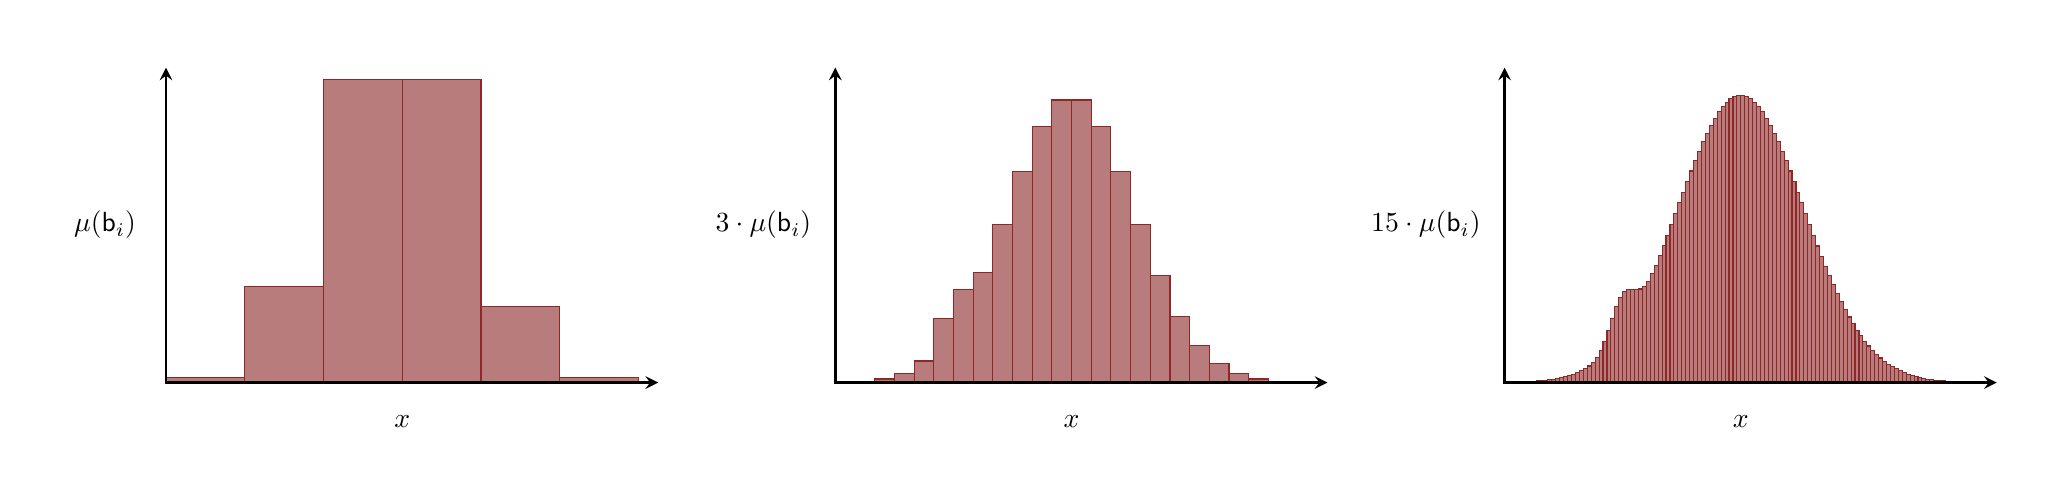
\begin{tikzpicture}[scale=1]
  \begin{scope}[shift={(0, 0)}]
    \draw[white] (-4.75, -3) rectangle (3.75, 2.5);
    
    \foreach \l/\u/\m in {-3.000000/-2.000000/0.005979, -2.000000/-1.000000/0.121933, -1.000000/0.000000/0.384502, 0.000000/1.000000/0.384491, 1.000000/2.000000/0.096954, 2.000000/3.000000/0.005968} {
      \filldraw[fill=mid, draw=dark] (\l, -2) rectangle (\u, {(10 * \m - 2)});
    }
    
    \draw[->, >=stealth, line width=1] (-3, -2.0175) -- (-3, +2);
    \draw[->, >=stealth, line width=1] (-3, -2) -- (+3.25, -2);
    \node at (0, -2.5) { $x$ };
    \node at (-4, 0) { $\hphantom{40 \cdot} \mu(\mathsf{b}_{i})$ };
  \end{scope}
  
  \begin{scope}[shift={(8.5, 0)}]
    \draw[white] (-4.75, -3) rectangle (3.75, 2.5);
    
    \foreach \l/\u/\m in {-3.000000/-2.750000/0.000200, -2.750000/-2.500000/0.000581, -2.500000/-2.250000/0.001530, -2.250000/-2.000000/0.003669, -2.000000/-1.750000/0.009124, -1.750000/-1.500000/0.026947, -1.500000/-1.250000/0.039277, -1.250000/-1.000000/0.046585, -1.000000/-0.750000/0.066897, -0.750000/-0.500000/0.089441, -0.500000/-0.250000/0.108561, -0.250000/0.000000/0.119603, 0.000000/0.250000/0.119603, 0.250000/0.500000/0.108561, 0.500000/0.750000/0.089441, 0.750000/1.000000/0.066886, 1.000000/1.250000/0.045401, 1.250000/1.500000/0.027972, 1.500000/1.750000/0.015642, 1.750000/2.000000/0.007940, 2.000000/2.250000/0.003658, 2.250000/2.500000/0.001530, 2.500000/2.750000/0.000581, 2.750000/3.000000/0.000200} {
      \filldraw[fill=mid, draw=dark] (\l, -2) rectangle (\u, {(30 * \m - 2)});
    }
    
    \draw[->, >=stealth, line width=1] (-3, -2.0175) -- (-3, +2);
    \draw[->, >=stealth, line width=1] (-3, -2) -- (+3.25, -2);
    \node at (0, -2.5) { $x$ };
    \node at (-4, 0) { $\hphantom{0}3 \cdot \mu(\mathsf{b}_{i})$ };
  \end{scope}
  
  \begin{scope}[shift={(17, 0)}]
    \draw[white] (-4.75, -3) rectangle (3.75, 2.5);
    
    \foreach \l/\u/\m in {-3.000000/-2.950000/0.000024, -2.950000/-2.900000/0.000030, -2.900000/-2.850000/0.000038, -2.850000/-2.800000/0.000048, -2.800000/-2.750000/0.000059, -2.750000/-2.700000/0.000074, -2.700000/-2.650000/0.000091, -2.650000/-2.600000/0.000112, -2.600000/-2.550000/0.000137, -2.550000/-2.500000/0.000167, -2.500000/-2.450000/0.000203, -2.450000/-2.400000/0.000246, -2.400000/-2.350000/0.000297, -2.350000/-2.300000/0.000357, -2.300000/-2.250000/0.000427, -2.250000/-2.200000/0.000509, -2.200000/-2.150000/0.000604, -2.150000/-2.100000/0.000715, -2.100000/-2.050000/0.000844, -2.050000/-2.000000/0.000996, -2.000000/-1.950000/0.001178, -1.950000/-1.900000/0.001407, -1.900000/-1.850000/0.001710, -1.850000/-1.800000/0.002127, -1.800000/-1.750000/0.002701, -1.750000/-1.700000/0.003465, -1.700000/-1.650000/0.004403, -1.650000/-1.600000/0.005437, -1.600000/-1.550000/0.006426, -1.550000/-1.500000/0.007217, -1.500000/-1.450000/0.007708, -1.450000/-1.400000/0.007901, -1.400000/-1.350000/0.007898, -1.350000/-1.300000/0.007856, -1.300000/-1.250000/0.007914, -1.250000/-1.200000/0.008155, -1.200000/-1.150000/0.008592, -1.150000/-1.100000/0.009195, -1.100000/-1.050000/0.009919, -1.050000/-1.000000/0.010723, -1.000000/-0.950000/0.011576, -0.950000/-0.900000/0.012462, -0.900000/-0.850000/0.013368, -0.850000/-0.800000/0.014285, -0.800000/-0.750000/0.015206, -0.750000/-0.700000/0.016123, -0.700000/-0.650000/0.017029, -0.650000/-0.600000/0.017916, -0.600000/-0.550000/0.018775, -0.550000/-0.500000/0.019599, -0.500000/-0.450000/0.020380, -0.450000/-0.400000/0.021109, -0.400000/-0.350000/0.021778, -0.350000/-0.300000/0.022382, -0.300000/-0.250000/0.022913, -0.250000/-0.200000/0.023364, -0.200000/-0.150000/0.023732, -0.150000/-0.100000/0.024012, -0.100000/-0.050000/0.024200, -0.050000/0.000000/0.024295, 0.000000/0.050000/0.024295, 0.050000/0.100000/0.024200, 0.100000/0.150000/0.024012, 0.150000/0.200000/0.023732, 0.200000/0.250000/0.023364, 0.250000/0.300000/0.022913, 0.300000/0.350000/0.022382, 0.350000/0.400000/0.021778, 0.400000/0.450000/0.021109, 0.450000/0.500000/0.020380, 0.500000/0.550000/0.019599, 0.550000/0.600000/0.018775, 0.600000/0.650000/0.017916, 0.650000/0.700000/0.017029, 0.700000/0.750000/0.016123, 0.750000/0.800000/0.015206, 0.800000/0.850000/0.014285, 0.850000/0.900000/0.013367, 0.900000/0.950000/0.012460, 0.950000/1.000000/0.011569, 1.000000/1.050000/0.010700, 1.050000/1.100000/0.009857, 1.100000/1.150000/0.009046, 1.150000/1.200000/0.008269, 1.200000/1.250000/0.007529, 1.250000/1.300000/0.006829, 1.300000/1.350000/0.006169, 1.350000/1.400000/0.005552, 1.400000/1.450000/0.004977, 1.450000/1.500000/0.004444, 1.500000/1.550000/0.003953, 1.550000/1.600000/0.003502, 1.600000/1.650000/0.003091, 1.650000/1.700000/0.002717, 1.700000/1.750000/0.002379, 1.750000/1.800000/0.002075, 1.800000/1.850000/0.001803, 1.850000/1.900000/0.001561, 1.900000/1.950000/0.001345, 1.950000/2.000000/0.001155, 2.000000/2.050000/0.000988, 2.050000/2.100000/0.000842, 2.100000/2.150000/0.000715, 2.150000/2.200000/0.000604, 2.200000/2.250000/0.000509, 2.250000/2.300000/0.000427, 2.300000/2.350000/0.000357, 2.350000/2.400000/0.000297, 2.400000/2.450000/0.000246, 2.450000/2.500000/0.000203, 2.500000/2.550000/0.000167, 2.550000/2.600000/0.000137, 2.600000/2.650000/0.000112, 2.650000/2.700000/0.000091, 2.700000/2.750000/0.000074, 2.750000/2.800000/0.000059, 2.800000/2.850000/0.000048, 2.850000/2.900000/0.000038, 2.900000/2.950000/0.000030, 2.950000/3.000000/0.000024} {
      \filldraw[fill=mid, draw=dark] (\l, -2) rectangle (\u, {(150 * \m - 2)});
    }
    
    \draw[->, >=stealth, line width=1] (-3, -2.0175) -- (-3, +2);
    \draw[->, >=stealth, line width=1] (-3, -2) -- (+3.25, -2);
    \node at (0, -2.5) { $x$ };
    \node at (-4, 0) { $15 \cdot \mu(\mathsf{b}_{i})$ };
  \end{scope}
  
\end{tikzpicture}

\end{document}  